\newcommand{\const}{\;\mathrm{const}\;}

\section{Theorie}

    In diesem Abschnitt sollen die theoretischen Grundlagen der Interferenz und die Funktionsweise
    des Interferometers erläutert werden.

\subsection{Die Interferenz von Licht}

    Für den vorliegenden Versuch ist ausschließlich die Welleneigenschaft von Licht relevant.
    In der Annahme,
    dass Licht eine elektromagnetische Welle ist,
    kann die Orts- und Zeitabhängigkeit der elektrischen Feldstärke durch eine ebene Welle ausgedrückt werden:
    \begin{equation}
        \label{eqn:EbeneWelle}
        \vec{E} = \vec{E_0} \cos(kx - \omega t - \delta) \; .
    \end{equation}
    Dabei ist $k = \frac{2 \pi}{\lambda}$ die Wellenzahl,
    über die sich auch die Wellenlänge $\lambda$ ausdrücken lässt.
    Die Größe $\omega$ bezeichnet die Kreisfrequenz und $\delta$ einen beliebigen Phasenwinkel,
    welcher die Position der Welle in der Periode angibt.\\
    Aufgrund des Superpositionsprinzips überlagern sich Wellen aus verschiedenen Lichtquellen.
    Die elektrische Feldstärke kann aufgrund ihrer hohen Frequenz nicht gemessen werden,
    allerdings ist die Intensität
    \begin{equation*}
        I = \const \lvert \vec{E} \rvert
    \end{equation*}
    als zeitlicher Mittelwert messbar. % ??
    Für die Überlagerung der Wellen ergibt sich eine Gesamtintensität von
    \begin{equation*}
        I_\text{ges} = 2 \const \vec{E_0}^2 (1 + \symup{cos(\delta_2 - \delta_1))}.
    \end{equation*}
    Es zeigt sich,
    dass sich zusätzlich ein Interferenzterm $ 2 \const \vec{E_0}^2 \cos(\delta_2 - \delta_1) $ ergibt,
    welcher bei $\delta_2 - \delta_1 = (2n + 1) \pi$ mit $n \in \symbb{N_0}$ verschwindet.
    Die Gesamtintensität kann sich abhängig von der Phase um $\pm 2 \const \vec{E_0}^2 $ vom Mittelwert unterscheiden. \\
    \\
    Interferenz zwischen Lichtwellen kann nur auftreten,
    wenn das Licht kohärent ist.
    Das bedeutet,
    dass alle Lichtwellen aus allen Quellen sich als eine einzelne Welle der Form in \autoref{eqn:EbeneWelle} darstellen lassen,
    wobei $k$, $\omega$ und $\delta$ fest sind.
    Es gibt im Gegensatz zu inkohärentem Licht also keine Phasenfluktuationen aufgrund einer festen Phase $\delta$.
    Die Fluktuationen entstehen dadurch,
    dass Elektronen in Atomen nicht gleichzeitig ihre überschüssige Energie in Form eines Wellenzuges emittieren.
    Es wird deshalb oft ein Laser verwendet,
    welcher im Gleichtakt emittiert.\\
    Für Interferenz bei einer konventionellen Lichtquelle muss der emittierte Lichtstrahl geteilt werden,
    damit über die Differenz der optischen Weglänge ein Phasenunterschied erzeugt wird.
    Der grundsätzliche Aufbau dafür ist in \autoref{fig:Lichtspaltung} gezeigt.

    \begin{figure}
        \centering
        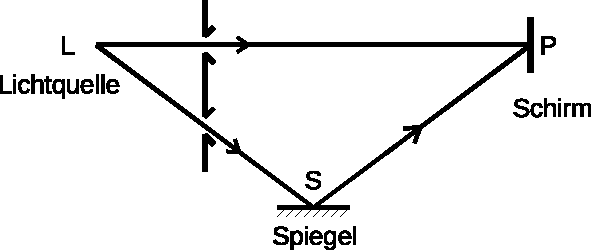
\includegraphics{content/img/Abb_1.pdf}
        \caption{Grundlegender Aufbau zur Spaltung eines Lichtstrahls. \cite{versuchsanleitung}}
        \label{fig:Lichtspaltung}
    \end{figure}

    Dabei wird der einfallende Lichtstrahl mithilfe einer Doppelblende in zwei Strahlenbündel aufgeteilt.
    Das eine Bündel bewegt sich ungehindert weiter,
    während das andere Bündel auf einen Spiegel trifft und reflektiert wird.
    Die Bündel treffen im Punkt \textbf{P} auf einem Schirm wieder zusammen.
    % komisch formuliert und jetzt redundant
    Aufgrund der Phasenverschiebung bei der Reflexion entsteht ein Wegunterschied $\Delta$ zwischen den Strahlbündeln
    und somit Interferenz.
    Der Wegunterschied verschwindet bei
    \begin{equation*}
        \Delta = (2n+1) \frac{\lambda}{2}
    \end{equation*}
    mit $n \in \symbb{N_0}$ und gleicher Feldstärke der Bündel.
    Er darf für Interferenz nicht größer sein als die endliche Länge des emittierten Wellenzuges,
    welche auf einer endlichen Zeit $\tau$,
    auch Kohärenzzeit genannt,
    der Emission gründet.
    Die Kohärenzlänge $l$ beschreibt mit
    \begin{equation*}
        l = N \lambda
    \end{equation*}
    genau den Wegunterschied,
    bei dem die Interferenz nicht mehr möglich ist.
    Die Zahl $N$ stellt die Anzahl der Intensitätsmaxima dar,
    die bei \textbf{P} beobachtet werden konnten.\\
    Ein weiteres Kriterium für Interferenz besteht also darin,
    dass der optische Wegunterschied zwischen den Wellenzügen nicht größer als die Kohärenzlänge sein darf.\\
    Nach dem Fourier'schen Theorem folgt,
    dass ein Wellenzug endlicher Länge ein Frequenz- bzw. Wellenlängenspektrum besitzt,
    also nicht perfekt monochromatisch und demnach nicht interferenzfähig ist.
    Es muss ein geringes Frequenzspektrum $\omega - \omega_0$ gewählt werden,
    damit die Maxima und Minima der Interferenz nicht zu sehr verwischt werden.
    %%%
    %TODO ↓ Das ist doch keine Frequenz, sondern die frequenzabhängige Amplitude,
    % also die Fourier-Transformierte, oder?
    Für die Frequenz eines sinusförmigen Wellenzuges endlicher Dauer gilt
    \begin{equation*}
        g(\omega) = 2 E_0 \frac{\sin(\omega - \omega_0) \frac{\tau}{2}}{\omega - \omega_0}
    \end{equation*}
    und demnach für die Intensität
    \begin{equation*}
        G(\omega) = \lvert g(\omega) \rvert ^2 = 4 {E_0}^2 \frac{\sin^2(\omega - \omega_0) \frac{{\tau}^2}{4}}{(\omega - \omega_0)^2} \ ,
    \end{equation*}
    sodass die Intensität bei $\omega_0$ maximal wird.
    %Sollen wir diesen Teil drinlassen? Ich finde zumindest das Fourier'sch Theorem wichtig, aber wir
    %benutzen die Gleichungen gar nicht ...
    %%%

\subsection{Funktionsweise des Michelson-Interferometers}

    Der Aufbau eines einfachen Interferometers ist in \autoref{fig:SchemaInterferometer} gezeigt.

    \begin{figure}
        \centering
        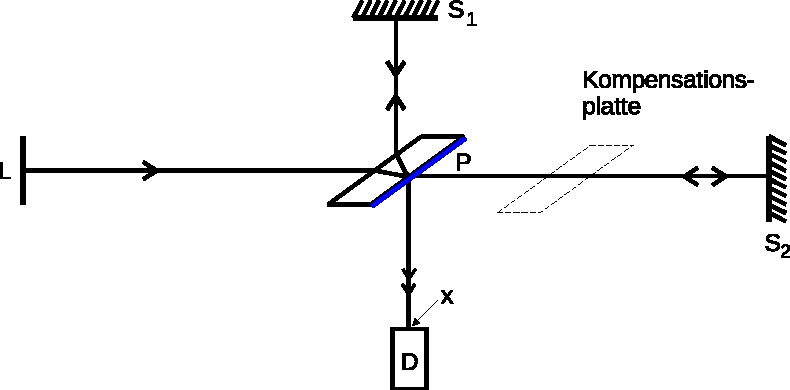
\includegraphics[width=0.75\textwidth]{content/img/Abb_4.pdf}
        \caption{Der Aufbau eines Interferometers. \cite{versuchsanleitung}}
        \label{fig:SchemaInterferometer}
    \end{figure}

    Hier wird der Lichtstrahl aus der Quelle \textbf{L} mithilfe einer semipermeablen Platte \textbf{P} geteilt.
    Ein Teil des Strahls wird von der Platte in eine senkrecht zur Einlaufrichtung stehende Richtung reflektiert,
    trifft auf einen Spiegel \textbf{S\textsubscript{1}} und wird dort erneut reflektiert.
    Der andere Teil läuft ungehindert durch die Platte hindurch und wird an einem Spiegel \textbf{S\textsubscript{2}} reflektiert.
    Damit der Wegunterschied der beiden Teilstrahlen kleiner als die Kohärenzlänge der Quelle ist,
    wird zwischen \textbf{P} und \textbf{S\textsubscript{2}} eine Kompensationsplatte eingebaut,
    mit derselben Dicke und demselben Brechungsindex wie \textbf{P}.
    Beide Teilstrahlen treffen wieder auf \textbf{P},
    wo ein Teil des Lichtes der beiden Strahlen parallel zueinander auf einen Detektor \textbf{D} trifft.
    Die Strecken zwischen \textbf{P} und \textbf{S\textsubscript{1}} und \textbf{S\textsubscript{2}} sollten fast gleich,
    dürfen allerdings nicht exakt gleich sein,
    da es sonst durch einen Gangunterschied von $\frac{\lambda}{2}$ aufgrund der Reflexion zu Auslöschung auf dem Weg zu \textbf{D} kommt.
    % TODO: Hier schon besser mit \Delta statt w?
    % "einer der Spiegel" ?
    Bei einer Verschiebung einer der Spiegel um $d$ ergibt sich ein Wegunterschied von $w = 2d$ zwischen den Strahlen,
    woraufhin sich die Intensität auf dem Detektorschirm verändert.
    Die Intensität kann mithilfe von
    \begin{equation*}
        I(d) = 2 \const \vec{E_0^2} \left( 1 + \cos\left( \frac{2\pi}{\lambda} 2d + \pi \right) \right)
    \end{equation*}
    berechnet werden.\\
    \\
    Mithilfe der kontinuierlichen Verschiebung eines Spiegels kann die Wellenlänge des genutzten Lichts gemessen werden.
    Der Spiegel wird dazu in Strahlrichtung mit einer Mikrometerschraube um $\symup{\Delta}d$ verschoben.
    Die Wellenlänge kann nun mit
    \begin{equation}
        \label{eqn:Wellenlänge}
        \lambda = \frac{2 \cdot \symup{\Delta}d}{z}
    \end{equation}
    berechnet werden,
    wobei $z$ die Anzahl der Intensitätsmaxima bezeichnet,
    die während der Verschiebung gezählt werden.\\
    Auf ähnliche Weise kann das Interferometer genutzt werden,
    um einen Brechungsindexunterschied $\symup{\Delta}n$ zu messen.
    Der optische Wegunterschied wird mithilfe eines Mediums der Länge $b$ und dem Brechungsindex $n + \symup{\Delta}n$ erzeugt.
    Der Brechungsindexunterschied kann durch
    \begin{equation}
        \label{eqn:brechungsindexunterschied}
        b \cdot \symup{\Delta}n = z \frac{\lambda}{2}
        % \symup{\Delta}n = \frac{z}{b} \frac{\lambda}{2}
    \end{equation}
    berechnet werden.
    Der optische Wegunterschied beträgt $b \cdot \symup{\Delta}n$
    und $z$ bezeichnet wie zuvor die Anzahl der auftretenden Intensitätsmaxima.

    \begin{figure}
        \centering
        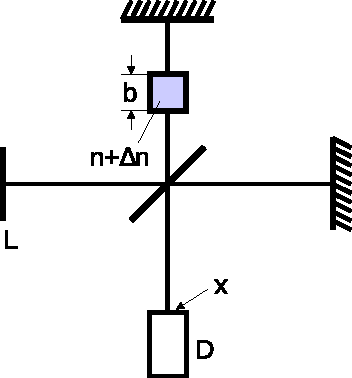
\includegraphics{content/img/Abb_5.pdf}
        \caption{Erweiterung des Aufbaus des Interferometers zur Messung von Brechungsindexunterschieden. \cite{versuchsanleitung}}
    \end{figure}

    Für die Messung von Gasen als Medium kann mithilfe der klassischen Dispersionstheorie der Zusammenhang
    \begin{equation*}
        n = \sqrt{1 + f(\lambda)N}
    \end{equation*}
    verwendet werden,
    wobei $N$ die Zahl der von der Lichtwelle angeregten Schwingungen von Dipolen pro Volumen darstellt.
    Zudem kann bei Gasen mit einem Druck von $\SI{0}{\bar}$ bis zu $\SI{1}{\bar}$ von einem idealen Gas ausgegangen werden und es gilt
    \begin{equation*}
        p V = R T .
    \end{equation*}
    Da $N(p,T)$ von der Temperatur $T$ und vom Druck $p$ abhängig ist,
    gilt
    \begin{align*}
        N(p,T) &= \frac{p}{T} \frac{T_0}{p_0} N_\text{L} & N(p',T) &= \frac{p'}{T} \frac{T_0}{p_0} N_\text{L}
    \end{align*}
    mit dem Normaldruck $p_0 = \SI{1013.3}{\bar}$,
    der Temperatur $T_0 = \SI{273.15}{\kelvin}$
    und der Loschmidt'schen Zahl $N_\text{L}$.
    Mithilfe einer Näherung ergibt sich mit der Brechungsindexänderung $\symup{\Delta}n(p,p')$ aus \autoref{eqn:brechungsindexunterschied}
    \begin{equation}
        \label{eqn:brechungsindex}
        n(p_0,T_0) = 1 + \symup{\Delta}n(p,p') \frac{T}{T_0} \frac{p_0}{p - p'}
    \end{equation}
    der Brechungsindex für das Gas unter Normalbedingungen.\\
    %Ich habe jetzt diese Formel genommen, weil ich keine Ahnung habe was f in der anderen ist.
    %Und das kann man ja umstellen.
    \\
    % Das passt hier nicht so richtig hin…
    Aufgrund der Verschiebung der Spiegel  % ←
    ändert sich der Wegunterschied zwischen den Strahlen,
    sodass es abwechselnd zu destruktiver und konstruktiver Interferenz kommt.
    Auf dem Schirm ist dies durch konzentrische Kreise erkennbar,
    wobei sich je nach Polarisation des Lichts veränderte Bilder ergeben können.
